% Provenance (never printed): SNT, "La photographie numerique" (photosites, sensor, demosaicing, image
% resolution, colour depth, metadata/EXIF, lossy and lossless processing); sound sampling and run-length coding are
% additions (sync ruling: Book 2 owns sampling rate and bit depth). See sources/book2/BRIEFS.md.
\chapter{Digital Images, Sound and Compression}\label{ch:g10:images-sound-compression}

Noor takes a photograph of the town square with her phone. The file on the phone weighs about $4$~MB. She sends the
picture to a friend in a message, and the copy that arrives weighs about $300$~KB, more than ten times less; on the
friend's screen it looks the same. Something was thrown away on the way, and something else was packed more
tightly.

\begin{omfigure}
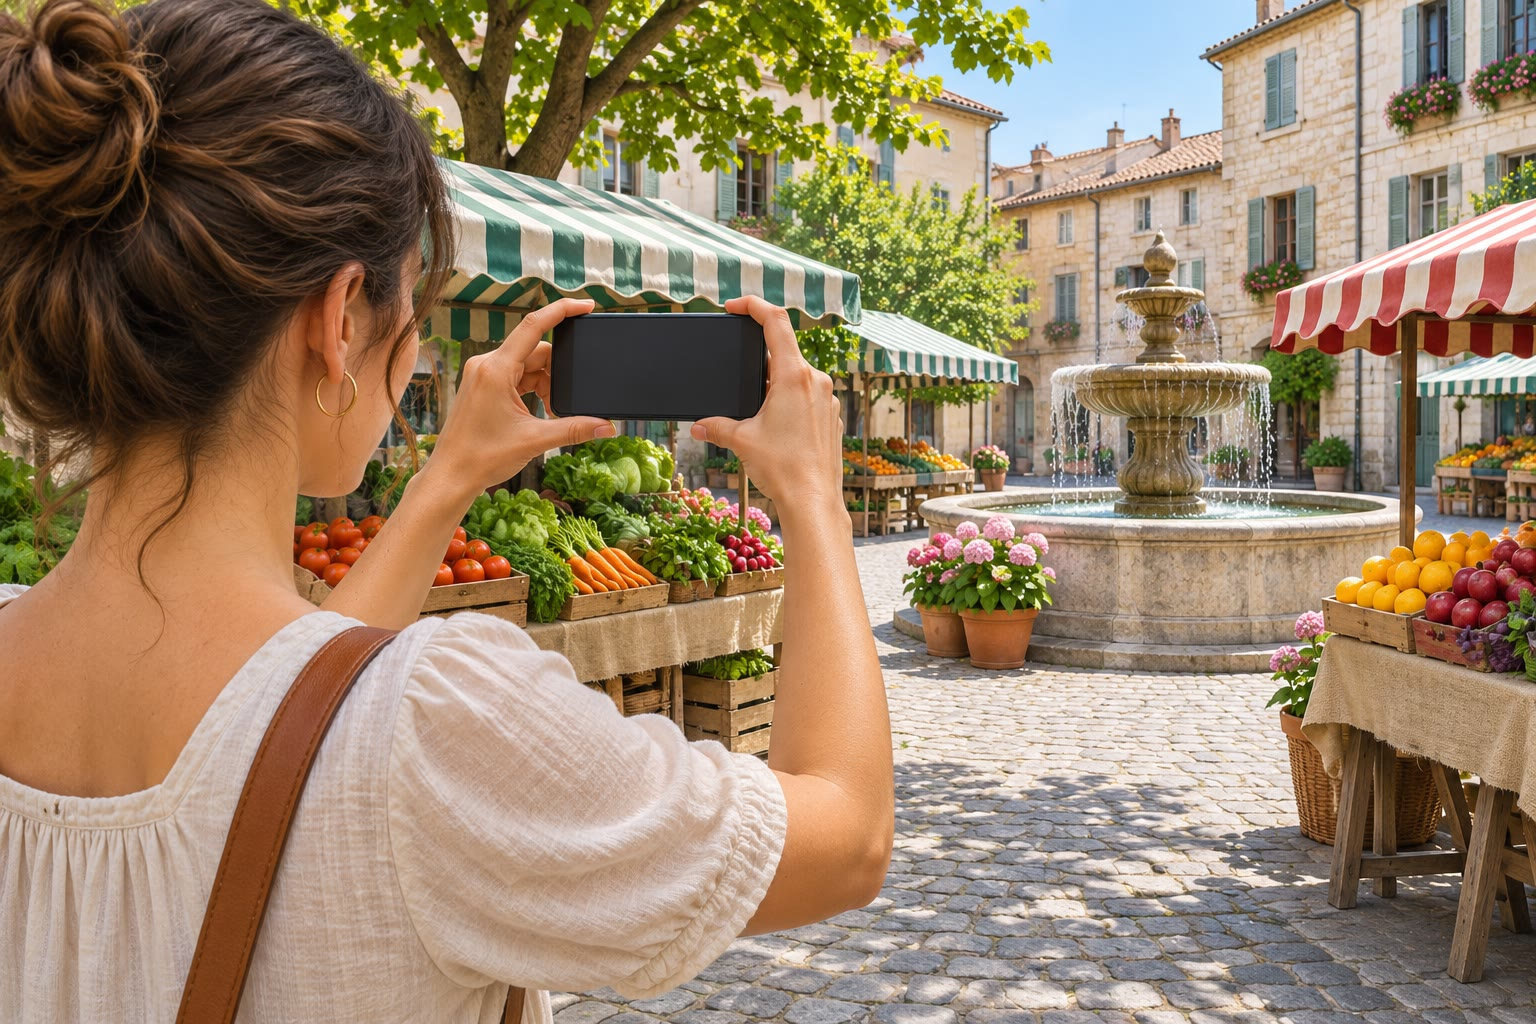
\includegraphics[width=0.55\linewidth]{images/book2/ai/g10-images-sound-compression-market.jpg}

{\small An illustration: taking a photograph of the market square, light becomes millions of numbers in a fraction of a
second.}
\end{omfigure}

This chapter follows a picture and a sound from the world into numbers: how a sensor measures light, how a microphone
signal becomes a list of samples, how big the raw numbers are, and the two ways of making them smaller, one that
loses nothing and one that loses what the eye or the ear will not miss.

\begin{recall}
An image on a screen is a grid of pixels, each with a red, a green and a blue value from $0$ to $255$ (Book 1,
grade 5); a grid image can be stored as a plain-text file of numbers (Book 1, grade 9). The resolution of an image is
its number of pixels across and down, and file sizes are counted in bytes, kilobytes and megabytes (Book 1, grade 4).
The physics book describes sound as a vibration of the air and a signal as a quantity that varies with time
(grade 10).
\end{recall}

\section{From a scene to pixels}\label{sec:g10:images-sound-compression:pixels}

A camera's sensor is a grid of millions of tiny light detectors.

\begin{omfigure}
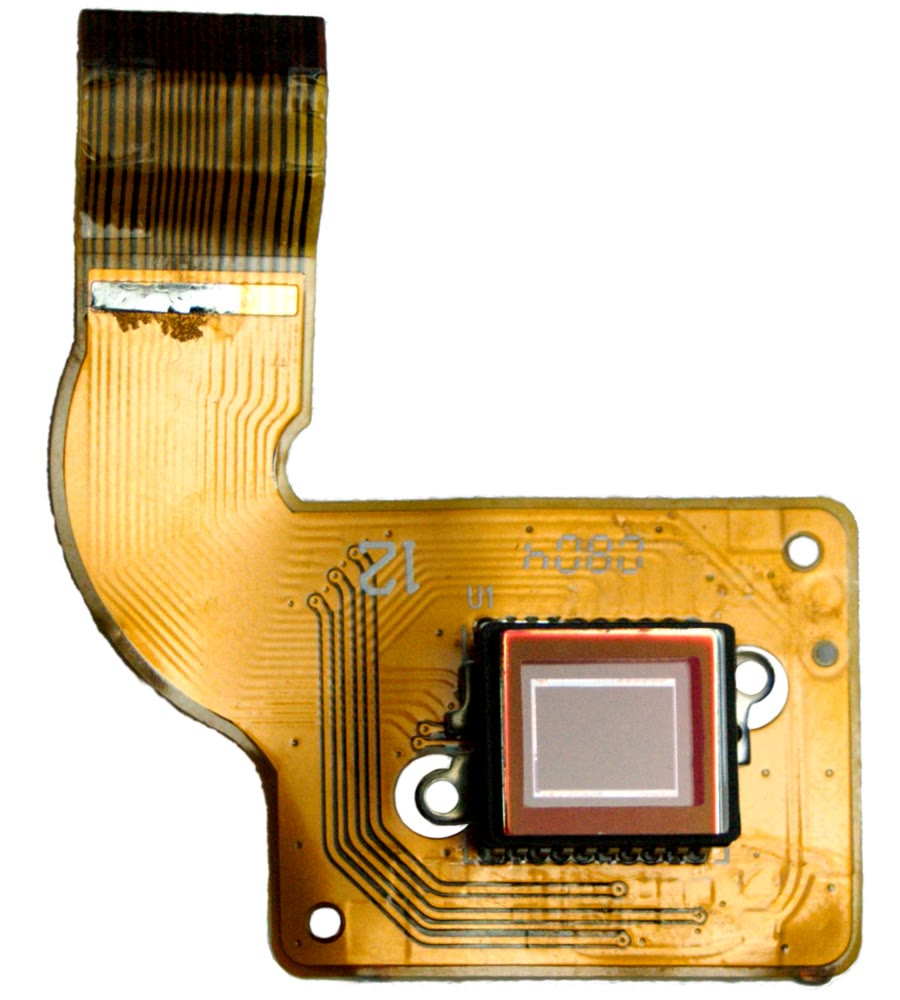
\includegraphics[width=0.36\linewidth]{images/book2/g10-image-sensor.jpg}

{\small The image sensor of a consumer digital camera, on its flexible circuit: the light falls on the rectangle in
the middle. Photograph: C-M, CC BY-SA 3.0.}
\end{omfigure}

\begin{definition}[Photosite]\label{def:g10:images-sound-compression:photosite}
A \emph{photosite}\index{photosite} is one light-sensitive cell of a camera's sensor. During the exposure it measures
how much light falls on it, as a number. A photosite measures brightness only; to see colour, each one sits under a
small red, green or blue filter and measures that colour alone.
\end{definition}

The filters form a repeating mosaic, usually with two green filters for one red and one blue in each $2 \times 2$
block, because the eye is most sensitive to green. A \omterm{def:g10:images-sound-compression:photosite}{photosite} therefore knows one of the three colours of its
pixel; the camera's processor guesses the other two from the neighbours. This step is called \emph{demosaicing}.

\begin{omfigure}
\begin{tikzpicture}[x=9mm, y=-9mm, font=\footnotesize]
  \foreach \r in {0,...,3} \foreach \c in {0,...,3} {
    \pgfmathtruncatemacro{\kind}{mod(\r,2)*2 + mod(\c,2)}
    \ifcase\kind \def\col{omThm!35}\def\lab{R}\or \def\col{omMeth!30}\def\lab{G}\or
      \def\col{omMeth!30}\def\lab{G}\or \def\col{omDef!35}\def\lab{B}\fi
    \fill[\col] (\c,\r) rectangle (\c+1,\r+1);
    \node at (\c+0.5,\r+0.5) {\lab};
  }
  \draw[step=1] (0,0) grid (4,4);
  \draw[ultra thick, omProp] (0,0) rectangle (3,3);
  \draw[ultra thick] (1,1) rectangle (2,2);
  \node[anchor=west, align=left, font=\footnotesize] at (4.4,1.5)
    {at the blue photosite (1, 1):\\red = average of the $4$ red corners\\green = average of the $4$ green sides\\
    blue = its own measurement};
\end{tikzpicture}

{\small A colour filter mosaic over $4 \times 4$ \omterm{def:g10:images-sound-compression:photosite}{photosites}, and the $3 \times 3$ neighbourhood used to give the blue
\omterm{def:g10:images-sound-compression:photosite}{photosite} at row $1$, column $1$ its missing red and green.}
\end{omfigure}

\omcode{code/grade-10/06-images-sound-compression/listings/demosaic.py}{1}{33}{Demosaicing by averaging the
neighbours.}\label{lst:g10:images-sound-compression:demosaic}

\omoutput{code/grade-10/06-images-sound-compression/outputs/demosaic.txt}{The mosaic, each value with the colour it
measured, and two pixels rebuilt.}\label{out:g10:images-sound-compression:demosaic}

Real cameras use cleverer guesses than a plain average, but the principle is the same: two thirds of the colour
values of a photograph were computed, not measured.

\begin{definition}[Colour depth]\label{def:g10:images-sound-compression:colour-depth}
The \emph{colour depth}\index{colour depth} of an image is the number of bits used for the colour of one pixel. With
one byte for each of red, green and blue, it is $24$ bits, which gives $2^{24} = 16{,}777{,}216$ colours.
\end{definition}

The raw size of an image follows: width times height times bytes per pixel.

\omcode{code/grade-10/06-images-sound-compression/listings/raw_size.py}{1}{9}{Raw sizes of three
images.}\label{lst:g10:images-sound-compression:raw-size}

\omoutput{code/grade-10/06-images-sound-compression/outputs/raw_size.txt}{A $12$-megapixel photograph takes $36$
million bytes before any \omterm{def:g10:images-sound-compression:compression}{compression}.}\label{out:g10:images-sound-compression:raw-size}

So Noor's $4$~MB file is already about nine times smaller than the raw $36$~MB of the image it holds.

\section{Sound as numbers}\label{sec:g10:images-sound-compression:sound}

A microphone turns the vibration of the air into an electric signal that varies continuously with time. A computer
keeps only some values of it.

\begin{definition}[Sampling rate, bit depth]\label{def:g10:images-sound-compression:sampling-rate}
To \emph{sample} a signal is to measure it at regular instants. The \emph{sampling rate}\index{sampling rate} is the
number of measurements, or \emph{samples}, per second, in hertz (Hz). Each sample is then rounded to one of a fixed
number of levels, a step called \emph{quantisation}; the \emph{bit depth}\index{bit depth} is the number of bits used
for one sample, so that there are $2^{\text{bit depth}}$ levels.
\end{definition}

\begin{omfigure}
\begin{tikzpicture}
  \begin{axis}[omrecord, width=0.85\linewidth, height=5cm, xlabel={time (ms)}, ylabel={signal},
      xmin=0, xmax=2.5, ymin=-1.15, ymax=1.15, ytick={-1,0,1}, legend pos=south west]
    \addplot[omDef, thick, smooth, domain=0:2.5, samples=200] {sin(deg(2*pi*0.44*x))};
    \addlegendentry{tone}
    \addplot[omProp, thick, const plot, mark=*, mark size=1.2pt]
      table[x=ms, y=level] {code/grade-10/06-images-sound-compression/figures/samples_plot.dat};
    \addlegendentry{samples, 8 levels}
  \end{axis}
\end{tikzpicture}

{\small A $440$~Hz tone sampled $8000$ times per second and quantised on $3$ bits, that is $8$ levels. Each dot is a
stored sample; between two samples nothing is kept. With $16$ bits the steps would be more than $9000$ times finer.}
\end{omfigure}

% ledger: g10:cd-44100-16
The audio compact disc samples $44{,}100$ times per second with $16$ bits per sample. A stereo recording keeps two
channels, one for each ear, so a second of it holds $44{,}100 \times 2 \times 2 = 176{,}400$ bytes. The listing
writes one second of a tone at a smaller rate and depth, with Python's \code{wave} module.

\omcode{code/grade-10/06-images-sound-compression/listings/make_wav.py}{1}{18}{One second of a $440$~Hz tone, $8$~kHz,
$8$ bits.}\label{lst:g10:images-sound-compression:make-wav}

\omoutput{code/grade-10/06-images-sound-compression/outputs/make_wav.txt}{$8000$ samples of one byte, and $44$ bytes
more for the file's header.}\label{out:g10:images-sound-compression:make-wav}

The values go up and down around $128$, the middle of a byte, once every $8000 / 440 \approx 18$ samples. A higher
\omterm{def:g10:images-sound-compression:sampling-rate}{sampling rate} follows faster vibrations, which the ear hears as higher notes; the physics book explains why a rate of
twice the highest frequency is needed.

\section{Compression without loss}\label{sec:g10:images-sound-compression:lossless}

\begin{definition}[Compression, lossless, lossy]\label{def:g10:images-sound-compression:compression}
\emph{Compression}\index{compression} encodes data in fewer bytes. It is \emph{lossless}\index{lossless} when
decompression gives back exactly the original bytes, and \emph{lossy}\index{lossy} when it gives back only an
approximation, chosen so that the difference is hard to notice.
\end{definition}

\begin{definition}[Compression ratio]\label{def:g10:images-sound-compression:ratio}
The \emph{compression ratio}\index{compression ratio} is the original size divided by the compressed size. A ratio of
$4$ means the compressed data is four times smaller; a ratio below $1$ means it grew.
\end{definition}

The simplest \omterm{def:g10:images-sound-compression:compression}{lossless} method works on data with long stretches of the same value, such as a map with a plain
background.

\begin{definition}[Run-length coding]\label{def:g10:images-sound-compression:rle}
\emph{Run-length coding}\index{run-length coding} replaces each \emph{run}, a maximal stretch of equal consecutive
values, by the pair (length of the run, value).
\end{definition}

\begin{omfigure}
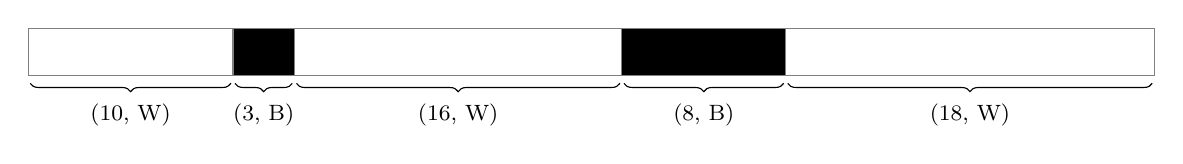
\begin{tikzpicture}[x=2.6mm, font=\footnotesize]
  \foreach \start/\len/\col in {0/10/white, 10/3/black, 13/16/white, 29/8/black, 37/18/white}
    \fill[\col, draw=black!50] (\start,0) rectangle (\start+\len,0.6);
  \draw[black!50] (0,0) rectangle (55,0.6);
  \foreach \start/\len/\lab in {0/10/{(10, W)}, 10/3/{(3, B)}, 13/16/{(16, W)}, 29/8/{(8, B)}, 37/18/{(18, W)}} {
    \draw[decorate, decoration={brace, amplitude=3pt, mirror}] (\start+0.1,-0.1) -- (\start+\len-0.1,-0.1)
      node[midway, below=4pt] {\lab};
  }
\end{tikzpicture}

{\small One row of $55$ pixels of a map, white and black, and its five runs. Ten numbers describe $55$ pixels.}
\end{omfigure}

\omcode{code/grade-10/06-images-sound-compression/listings/rle.py}{1}{27}{\omterm{def:g10:images-sound-compression:rle}{Run-length coding}, on a map row and on
noise.}\label{lst:g10:images-sound-compression:rle}

\omoutput{code/grade-10/06-images-sound-compression/outputs/rle.txt}{Five runs for the map row; $21$ for a random
row of the same length.}\label{out:g10:images-sound-compression:rle}

On noise the runs are short, and storing each one as a pair can take more room than the pixels themselves. How much
a method compresses depends on the data, not only on the method.

% ledger: g10:deflate-1996
The general-purpose compressors used for files, such as the DEFLATE method behind \code{zip} files and Python's
\code{zlib} module (described in 1996), go further: they replace a repeated sequence by a reference to its earlier
occurrence, a \emph{dictionary method}, and write frequent values with fewer bits than rare ones.

\omcode{code/grade-10/06-images-sound-compression/listings/zlib_sizes.py}{1}{13}{\code{zlib} on three kinds of
data.}\label{lst:g10:images-sound-compression:zlib-sizes}

\omoutput{code/grade-10/06-images-sound-compression/outputs/zlib_sizes.txt}{Repetitive data shrinks a hundredfold;
random bytes grow a little.}\label{out:g10:images-sound-compression:zlib-sizes}

\begin{proposition}[No lossless method shrinks everything]\label{prop:g10:images-sound-compression:no-universal}
For every \omterm{def:g10:images-sound-compression:compression}{lossless} \omterm{def:g10:images-sound-compression:compression}{compression} method and every $n$, some file of $n$ bytes is not made shorter.
\end{proposition}

The proof is \cref{exo:g10:images-sound-compression:12}: it counts files. The random bytes of the listing are such
files, and so, very nearly, are recordings of music, as the weekend problem shows.

\section{Compression with loss}\label{sec:g10:images-sound-compression:lossy}

A photograph or a song does not have to come back bit for bit: it has to look or sound the same. \omterm{def:g10:images-sound-compression:compression}{Lossy} methods throw
away what matters least: fine detail that the eye cannot see at the viewing size, sounds hidden by louder ones, and
small differences of colour or loudness. The simplest of these steps uses fewer levels.

\omcode{code/grade-10/06-images-sound-compression/listings/quantise.py}{1}{12}{Fewer grey
levels.}\label{lst:g10:images-sound-compression:quantise}

\omoutput{code/grade-10/06-images-sound-compression/outputs/quantise.txt}{With $8$ levels instead of $256$, each grey
needs $3$ bits instead of $8$, and is off by at most $18$.}\label{out:g10:images-sound-compression:quantise}

\begin{omfigure}
\begin{tikzpicture}[font=\footnotesize, node distance=9mm, s/.style={draw, rounded corners=2pt, minimum height=8mm,
    inner sep=3pt, align=center}]
  \node[s, fill=omDef!8] (o) {original\\$36$ MB};
  \node[s, right=of o] (l1) {throw away\\what is not seen};
  \node[s, right=of l1] (l2) {pack tightly\\(lossless)};
  \node[s, right=of l2, fill=omProp!14] (c) {file\\$0.3$ to $4$ MB};
  \draw[ptr] (o) -- (l1); \draw[ptr] (l1) -- (l2); \draw[ptr] (l2) -- (c);
  \node[below=2mm of l1, text=omProp, align=center] {lossy:\\cannot be undone};
  \node[below=2mm of l2, text=omDef, align=center] {lossless:\\undone exactly};
\end{tikzpicture}

{\small How a photograph file is made: a \omterm{def:g10:images-sound-compression:compression}{lossy} step chooses what to forget, then a \omterm{def:g10:images-sound-compression:compression}{lossless} step packs what is left.
Sending a picture in a message usually repeats the \omterm{def:g10:images-sound-compression:compression}{lossy} step more strongly.}
\end{omfigure}

\begin{method}[Choosing a kind of compression]\label{met:g10:images-sound-compression:choose}
\begin{enumerate}
  \item Programs, text, tables and anything that must come back exactly: \omterm{def:g10:images-sound-compression:compression}{lossless} only.
  \item Photographs, music and video meant for eyes and ears: \omterm{def:g10:images-sound-compression:compression}{lossy}, at a quality chosen for the use (a message, a
    print, an archive).
  \item Never compress a \omterm{def:g10:images-sound-compression:compression}{lossy} file again and again with loss: each round loses a little more.
\end{enumerate}
\end{method}

\section{Metadata}\label{sec:g10:images-sound-compression:metadata}

\begin{definition}[Metadata]\label{def:g10:images-sound-compression:metadata}
The \emph{metadata}\index{metadata} of a file is data about the data it holds: for an image, its width, height and
\omterm{def:g10:images-sound-compression:colour-depth}{colour depth}; for a sound, its \omterm{def:g10:images-sound-compression:sampling-rate}{sampling rate}, \omterm{def:g10:images-sound-compression:sampling-rate}{bit depth} and number of channels; often also the date, the device and
the place where it was made.
\end{definition}

Every image or sound file starts with a \emph{header} that holds the \omterm{def:g10:images-sound-compression:metadata}{metadata} a program needs to read the rest.
% ledger: g10:ppm-header, g10:wave-riff
The simple PPM image format writes its header as text: the letters \code{P6}, the width, the height and the largest
value. A WAV file, a format of 1991, starts with the four letters \code{RIFF}, then \code{WAVE} and a block named
\code{fmt } that gives the channels, the \omterm{def:g10:images-sound-compression:sampling-rate}{sampling rate} and the \omterm{def:g10:images-sound-compression:sampling-rate}{bit depth}.

\omcode{code/grade-10/06-images-sound-compression/listings/read_header.py}{1}{18}{Writing two tiny files and reading
their headers.}\label{lst:g10:images-sound-compression:read-header}

\omoutput{code/grade-10/06-images-sound-compression/outputs/read_header.txt}{$2 \times 2$ pixels take $12$ bytes and
the PPM header $11$; the WAV file begins with its format's name.}\label{out:g10:images-sound-compression:read-header}

\begin{safety}
A photograph taken with a phone usually carries, in its \omterm{def:g10:images-sound-compression:metadata}{metadata}, the date, the model of the phone and often the
exact position where it was taken. Before sharing a picture of a place that should stay private, such as your home,
check what the file says about itself, or use a program or setting that removes the \omterm{def:g10:images-sound-compression:metadata}{metadata}.
\end{safety}

\section{Exercises}\label{sec:g10:images-sound-compression:exercises}

\begin{exercise}[$\star$]\label{exo:g10:images-sound-compression:1}
What is the raw size, in bytes and in MiB, of a $4000 \times 3000$ image with $3$ bytes per pixel? And of the same
image in grey levels with one byte per pixel?
\end{exercise}

\begin{exercise}[$\star$]\label{exo:g10:images-sound-compression:2}
How many bytes does one second of stereo sound take at $48{,}000$ samples per second and $16$ bits per sample? And one
hour?
\end{exercise}

\begin{exercise}[$\star$]\label{exo:g10:images-sound-compression:3}
What does \code{rle_encode("AAABCCCCD")} return? How many numbers and characters does the result hold, against the
$9$ characters of the string?
\end{exercise}

\begin{exercise}[$\star$]\label{exo:g10:images-sound-compression:4}
Put these in order of compressed size with \code{zlib}, without running: $10{,}000$ copies of the letter \code{a}; a
book chapter of $10{,}000$ characters; $10{,}000$ random bytes. Explain.
\end{exercise}

\begin{exercise}[$\star$]\label{exo:g10:images-sound-compression:5}
Write \code{rle_decode(runs)} without looking at the listing, and check that decoding an encoding gives back the
string.
\end{exercise}

\begin{exercise}[$\star\star$]\label{exo:g10:images-sound-compression:6}
An encoder walks through the string with an index, counts equal neighbours, and appends a run each time the character
changes. On \code{"WWB"} it returns \code{[(2, "W")]}. Find the bug and correct it; which strings does the buggy
version handle correctly?
\end{exercise}

\begin{exercise}[$\star\star$]\label{exo:g10:images-sound-compression:7}
Suppose a run is stored in $2$ bytes, one for the length and one for the value. Which row of $n$ pixels of one byte
each makes the encoding as long as possible, and how long? When does \omterm{def:g10:images-sound-compression:rle}{run-length coding} pay?
\end{exercise}

\begin{exercise}[$\star\star$]\label{exo:g10:images-sound-compression:8}
A plain PGM image is a text file: \code{P2}, the width, the height, the largest grey value, then the grey values.
Write \code{histogram(text)}, which returns the list of the numbers of pixels of each grey level.
\end{exercise}

\begin{exercise}[$\star\star$]\label{exo:g10:images-sound-compression:9}
Some screens store a colour in $16$ bits: $5$ for red, $6$ for green and $5$ for blue. How many colours is that? How
many levels does each colour have, and why might green get the extra bit?
\end{exercise}

\begin{exercise}[$\star\star$]\label{exo:g10:images-sound-compression:10}
A student changes the condition of the demosaicing listing to \code{0 <= rr <= 4 and 0 <= cc <= 4}. Which pixels
does this break, and how?
\end{exercise}

\begin{exercise}[$\star\star$]\label{exo:g10:images-sound-compression:11}
Write \code{wav_duration(path)}, which returns the duration of a WAV file in seconds from the number of frames and the
\omterm{def:g10:images-sound-compression:sampling-rate}{sampling rate} in its header. What is the duration of the tone of the listing?
\end{exercise}

\begin{exercise}[$\star\star\star$]\label{exo:g10:images-sound-compression:12}
Prove the proposition that no \omterm{def:g10:images-sound-compression:compression}{lossless} method shrinks every file: count the files of exactly $n$ bytes, and the files
of fewer than $n$ bytes, and use the fact that two different files must not be compressed to the same result.
\end{exercise}

\begin{exercise}[$\star\star\star$]\label{exo:g10:images-sound-compression:13}
Write \code{bitmap_ratio(rows)} for a black-and-white bitmap given as a list of strings of \code{W} and \code{B}: it
returns the number of pixels, the number of runs over all rows, and the ratio when each run costs as much as two
pixels. Try it on a bitmap of your own with large plain areas, and on a chessboard.
\end{exercise}

\begin{exercise}[$\star\star\star$]\label{exo:g10:images-sound-compression:14}
Prove that rounding a grey value to the nearest of evenly spaced levels with step $s$ makes an error of at most
$s/2$. Check it against the output of the quantisation listing for $16$ and $8$ levels.
\end{exercise}

\begin{exercise}[$\star\star\star$]\label{exo:g10:images-sound-compression:15}
A tone of $7000$~Hz is sampled $8000$ times per second. Count, in the samples, how many times per second the signal
goes from negative to non-negative. What frequency does the recording seem to have? Explain with the positions of the
samples on the wave (this effect is called \emph{aliasing}).
\end{exercise}

\section{Problem: A Minute of Music}\label{sec:g10:images-sound-compression:problem}

\begin{problem}[{Weekend problem --- why music files hardly shrink with a general-purpose compressor}]\label{pb:g10:images-sound-compression:1}
A disc-quality recording uses the compact disc's \omterm{def:g10:images-sound-compression:sampling-rate}{sampling rate} and \omterm{def:g10:images-sound-compression:sampling-rate}{bit depth}, in stereo. The program
\code{exercises/minute_of_music.py} computes its size and compresses one second of synthetic music, made of three
tones and a little noise, and one second of silence.

\needspace{4\baselineskip}\medskip\noindent\textbf{Part I --- The format.}
\begin{enumerate}
  \item Give the \omterm{def:g10:images-sound-compression:sampling-rate}{sampling rate} and the \omterm{def:g10:images-sound-compression:sampling-rate}{bit depth} of the compact disc.
  \item How many levels can one sample take?
  \item How many samples does one second of stereo hold?
  \item How long is the gap between two samples of one channel, in microseconds?
\end{enumerate}

\needspace{4\baselineskip}\medskip\noindent\textbf{Part II --- Bytes per second and per minute.}
\begin{enumerate}[resume]
  \item Compute the number of bytes per second.
  \item Compute the number of bytes per minute.
  \item Convert it to MiB ($1$~MiB $= 2^{20}$ bytes) and to MB ($10^6$ bytes).
  \item What is the bit rate, in bits per second?
\end{enumerate}

\needspace{4\baselineskip}\medskip\noindent\textbf{Part III --- A song and an album.}
\begin{enumerate}[resume]
  \item What is the raw size of a song of $3$ minutes $30$ seconds?
  \item How many such songs fit in $1$~GB ($10^9$ bytes)?
  \item A WAV file adds a header of $44$ bytes. By what fraction does it change the size of the song?
  \item A music service sends the same song at $160{,}000$ bits per second. What is its \omterm{def:g10:images-sound-compression:ratio}{compression ratio} against the
    raw recording?
  \item Is that \omterm{def:g10:images-sound-compression:compression}{compression} \omterm{def:g10:images-sound-compression:compression}{lossy} or \omterm{def:g10:images-sound-compression:compression}{lossless}? Use the proposition of this chapter and Part IV to argue.
\end{enumerate}

\needspace{4\baselineskip}\medskip\noindent\textbf{Part IV --- Compressing samples.}
\begin{enumerate}[resume]
  \item Run the program. How many runs does one second of music have, against how many bytes? What would \omterm{def:g10:images-sound-compression:rle}{run-length
    coding} do to it?
  \item What ratio does \code{zlib} reach on the music, and on the silence?
  \item Why are the bytes of music so different from one to the next, even for a smooth tone? Think of what a $16$-bit
    sample's low byte holds.
  \item Why does the silence compress so well?
  \item A recording has a long silence at the end. Explain why \omterm{def:g10:images-sound-compression:compression}{lossless} \omterm{def:g10:images-sound-compression:compression}{compression} of the whole file still gains a
    little.
  \item State the result: the size of one minute of disc-quality stereo, in bytes and in MiB, and the ratio that
    \code{zlib} reaches on music against silence.
\end{enumerate}
\end{problem}
